% This is samplepaper.tex, a sample chapter demonstrating the
% LLNCS macro package for Springer Computer Science proceedings;
% Version 2.20 of 2017/10/04
%
%\documentclass[runningheads]{llncs}
%
\documentclass[10pt,a4paper]{article}
\usepackage{hyperref}
\renewcommand\UrlFont{\color{blue}\rmfamily}
\setlength{\parskip}{0pt}
\raggedbottom
\usepackage{multirow}
\usepackage{amsmath}
\usepackage{csquotes}
\usepackage{paralist}
\usepackage{booktabs}
\usepackage{mathptmx}
\usepackage{pgfplots}
\pgfplotsset{compat=1.8}
\usepackage{subfigure}
\usepackage{pgfplots}
\pgfplotsset{width=7cm,compat=1.8}
\usepackage{pgfplotstable}
\renewcommand*{\familydefault}{\sfdefault}
\usepackage{tikz}
%\pgfplotset{compact=1.16 }
\begin{document}
Table 1  below shows the performance measures (precision, recall, F measure and precision) of the results of our Decision Tree classifier after experimentation on all our datasets. The observation shows that the best scores of our classifier are achieved on the datasets DT1, DT3 and DT5 which are 97.04\%, 80.86\% and 83.41\% respectively. Noticing that sensitivity values are higher than specificity values for Also AUC (Area Under the Curve) values are higher for these same datasets which are 0.78, 0.86 and 0.76 respectively. However, we note that the sensitivity values are higher than the specificity values on the datasets DT1 and DT5 so that they are substantially identical for the datasets DT2, DT3 and DT4. This means that DT is more inclined to predict as well whether a given patient has malaria or he doesn’t, on the datasets DT2, DT3 and DT4, while our classifier on the datasets DT1 and DT5 our classifier is only efficient in predicting whether a given patient has malaria. This same trend is observed on the F-scores which higher values varying between 0.91 and 0.98 on the datasets DT1, DT3 and DT5.
% Decision Tree
\begin{center}
\textbf{Decision Tree}
\end{center}

\begin{table}[!ht]
\centering
\begin{tabular}{*{6}{c}l r}
  \toprule
  \textbf{Datasets} & \textbf{Precision} & \textbf{Recall} & \textbf{F1-score}&\textbf{AUC} &\textbf{Score}\\
   \midrule
  DT1 &0.97 & 1  & 0.98& 0.78&97.04 \\
  DT2 & 0.59 &0.48&0.48&0.64&63.01 \\
  DT3 &0.89 &0.85 &0.87&0.86&80.86\\
  DT4 &0.68 &0.57&0.62&0.70&65.60\\
  DT5 &0.99 &0.84&0.91&0.76&83.41\\

  
    \bottomrule
\end{tabular}
\caption{Performances measures of DT over all datasets}\label{perf-measure-dt1}
\end{table}

%Random Forest
\begin{center}
\textbf{Random Forest}
\end{center}
\begin{table}[!ht]
\centering
\begin{tabular}{*{6}{c}l r}
  \toprule
  \textbf{Datasets} & \textbf{Precision} & \textbf{Recall} & \textbf{F1-score}&\textbf{AUC} &\textbf{Score}\\
   \midrule
  DT1 &0.97 &1   &0.99 &0.81 &97.13 \\
  DT2 &0.63  & 0.34  &0.44&0.64&63.33 \\
  DT3 &0.89 &0.85 &0.87&087&80.86\\
  DT4 &0.68 &0.56&0.62&0.70&65.82\\
  DT5 &0.99 &0.84&0.91&0.76&78.35\\
  
  
    \bottomrule
\end{tabular}
\caption{Performances measures of RF over all datasets}\label{perf-measure-dt1}
\end{table}


%Logistic Regression
\begin{center}
\textbf{Logistic Regression}
\end{center}
\begin{table}[!ht]
\centering
\begin{tabular}{*{6}{c}l r}
  \toprule
  \textbf{Datasets} & \textbf{Precision} & \textbf{Recall} & \textbf{F1-score}&\textbf{AUC} &\textbf{Score}\\
   \midrule
  DT1 &0.97 &1   &0.99 &0.79 &97.19 \\
  DT2 & 0.58 &0.36   &0.44&0.63&61.96\\
  DT3 &0.85 &0.88 &0.86&0.86&79.59\\
  DT4 &0.98 &0.56&0.92&0.70&65.82\\
  DT5 & 0.90&0.78&0.88&0.84&81.86\\
  
  
    \bottomrule
\end{tabular}
\caption{Performances measures of LR over all datasets}\label{perf-measure-dt1}
\end{table}
\newpage
%Naives Bayes
\begin{center}
\textbf{Naives Bayes}

\end{center}
\begin{table}[!ht]
\centering
\begin{tabular}{*{6}{c}l r}
  \toprule
  \textbf{Datasets} & \textbf{Precision} & \textbf{Recall} & \textbf{F1-score}&\textbf{AUC} &\textbf{Score}\\
   \midrule
  DT1 &0.97 &1   &0.99 &0.81 &97.13 \\
  DT2 & 0.60 &0.34   &0.43&0.63&62.86 \\
  DT3 &0.86 &0.87 &0.86&0.85&79.94\\
  DT4 &0.68 &0.59&0.63&0.70&65.63\\
  DT5 &0.99 &0.82&0.90&0.84&85.61\\
  
  
    \bottomrule
\end{tabular}
\caption{Performances measures of NB over all datasets}\label{perf-measure-dt1}
\end{table}

%SVM
\begin{center}
\textbf{SVM}

\end{center}
\begin{table}[!ht]
\centering
\begin{tabular}{*{6}{c}l r}
  \toprule
  \textbf{Datasets} & \textbf{Precision} & \textbf{Recall} & \textbf{F1-score}&\textbf{AUC} &\textbf{Score}\\
   \midrule
  DT1 &0.97 &1   &0.99 &.84 &97.13 \\
  DT2 &0.58  &0.05   & 0.09&0.62&62.86\\
  DT3 &0.57 & 0.86&0.86&0.85&79.94\\
  DT4 & 0.68&0.58&0.62&0.70&65.63\\
  DT5 &0.99 &0.86&0.92&0.80&85.61\\
    \bottomrule
\end{tabular}
\caption{Performances measures of SVM over all datasets}\label{perf-measure-dt1}
\end{table}
%ANN
\begin{center}
\textbf{ANN}
\end{center}
\begin{table}[!ht]
\centering
\begin{tabular}{*{6}{c}l r}
  \toprule
  \textbf{Datasets} & \textbf{Precision} & \textbf{Recall} & \textbf{F1-score}&\textbf{AUC} &\textbf{Score}\\
   \midrule
  DT1 0.97&1 &0.99   &0.84 &97.15  \\
  DT2 &0.59  &0.40   &0.48&0.65&62.86 \\
  DT3 &0.89 &0.85 &0.87&0.87&86.68\\
  DT4 &0.68 &0.58&0.62&0.70&0.70\\
  DT5 &0.99 &0.84&0.91&0.79&83.26\\ 
    \bottomrule
\end{tabular}
\caption{Performances measures of ANN over all datasets}\label{perf-measure-dt1}
\end{table}
\begin{table}
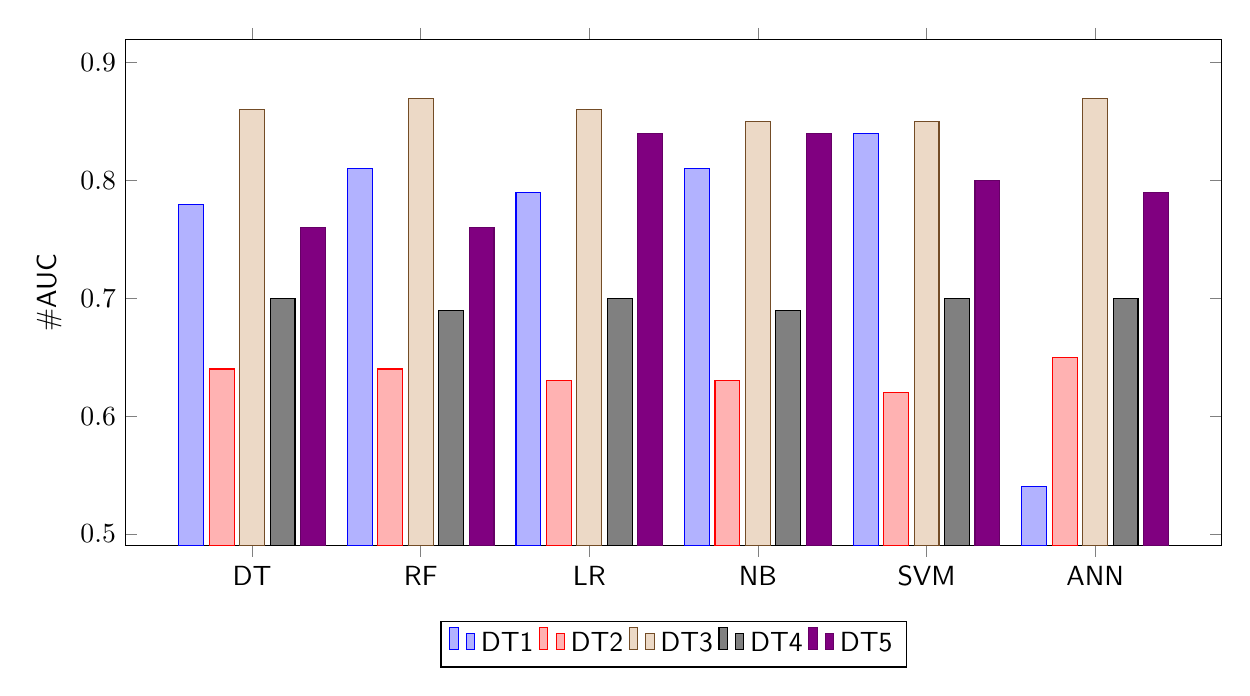
\begin{tikzpicture}
 \centering
\begin{axis}[
    height=8cm, width=15.5cm,
    bar width=0.4cm,
    ybar,
    %ybar=5pt,% configures `bar shift'
    bar width=9pt,
    enlargelimits=0.15,
    legend style={at={(0.5,-0.15)},
      anchor=north,legend columns=-1},
    ylabel={\#AUC},
    symbolic x coords={{DT,RF,LR,NB,SVM,ANN}},
    xtick=data,
    %nodes near coords,
    nodes near coords align={vertical},
    ]
\addplot coordinates {(DT,0.78) (RF, 0.81) (LR,0.79)(NB, 0.81)(SVM,0.84)(ANN, 0.54)};
\addplot coordinates{(DT,0.64) (RF, 0.64) (LR,0.63)(NB, 0.63)(SVM,0.62)(ANN, 0.65)};
\addplot coordinates {(DT,0.86) (RF, 0.87) (LR,0.86)(NB, 0.85)(SVM,0.85)(ANN, 0.87)};
\addplot coordinates {(DT,0.70) (RF, 0.69) (LR,0.70)(NB, 0.69)(SVM,0.70)(ANN, 0.70)};
\addplot coordinates {(DT,0.76) (RF, 0.76) (LR,0.84)(NB, 0.84)(SVM,0.80)(ANN, 0.79)};
\legend{DT1,DT2,DT3,DT4,DT5}
\end{axis}
\end{tikzpicture}
\caption{Performances measures of ANN over all datasets}\label{perf-measure-dt1}
\end{table}
\end{document}
